% !TEX TS-program = XeLaTeX
% use the following command: 
% all document files must be coded in UTF-8
\documentclass{textolivre}
% for anonymous submission
%\documentclass[anonymous]{textolivre}
% to create HTML use 
%\documentclass{textolivre-html}
% See more information on the repository: https://github.com/leolca/textolivre

% Metadata
\begin{filecontents*}[overwrite]{article.xmpdata}
    \Title{Effectiveness of flipped learning and augmented reality in the new educational normality of the Covid-19 era}
    \Author{Santiago Pozo-Sánchez \sep Jesús Lopez-Belmonte \sep Antonio José Moreno-Guerrero \sep Arturo Fuentes-Cabrera}
    \Language{en}
    \Keywords{ICT \sep Flipped learning \sep Augmented reality \sep Active methodologies \sep Educative technology}
    \Journaltitle{Texto Livre}
    \Journalnumber{1983-3652}
    \Volume{14}
    \Issue{2}
    \Firstpage{1}
    \Lastpage{16}
    \Doi{10.35699/1983-3652.2021.34260}

    \setRGBcolorprofile{sRGB_IEC61966-2-1_black_scaled.icc}
            {sRGB_IEC61966-2-1_black_scaled}
            {sRGB IEC61966 v2.1 with black scaling}
            {http://www.color.org}
\end{filecontents*}

% used to create dummy text for the template file
\definecolor{dark-gray}{gray}{0.35} % color used to display dummy texts
\usepackage{lipsum}
\SetLipsumParListSurrounders{\colorlet{oldcolor}{.}\color{dark-gray}}{\color{oldcolor}}

% used here only to provide the XeLaTeX and BibTeX logos
\usepackage{hologo}

% used in this example to provide source code environment
%\crefname{lstlisting}{lista}{listas}
%\Crefname{lstlisting}{Lista}{Listas}
%\usepackage{listings}
%\renewcommand\lstlistingname{Lista}
%\lstset{language=bash,
        breaklines=true,
        basicstyle=\linespread{1}\small\ttfamily,
        numbers=none,xleftmargin=0.5cm,
        frame=none,
        framexleftmargin=0.5em,
        framexrightmargin=0.5em,
        showstringspaces=false,
        upquote=true,
        commentstyle=\color{gray},
        literate=%
           {á}{{\'a}}1 {é}{{\'e}}1 {í}{{\'i}}1 {ó}{{\'o}}1 {ú}{{\'u}}1 
           {à}{{\`a}}1 {è}{{\`e}}1 {ì}{{\`i}}1 {ò}{{\`o}}1 {ù}{{\`u}}1
           {ã}{{\~a}}1 {ẽ}{{\~e}}1 {ĩ}{{\~i}}1 {õ}{{\~o}}1 {ũ}{{\~u}}1
           {â}{{\^a}}1 {ê}{{\^e}}1 {î}{{\^i}}1 {ô}{{\^o}}1 {û}{{\^u}}1
           {ä}{{\"a}}1 {ë}{{\"e}}1 {ï}{{\"i}}1 {ö}{{\"o}}1 {ü}{{\"u}}1
           {Á}{{\'A}}1 {É}{{\'E}}1 {Í}{{\'I}}1 {Ó}{{\'O}}1 {Ú}{{\'U}}1
           {À}{{\`A}}1 {È}{{\`E}}1 {Ì}{{\`I}}1 {Ò}{{\`O}}1 {Ù}{{\`U}}1
           {Ã}{{\~A}}1 {Ẽ}{{\~E}}1 {Ũ}{{\~u}}1 {Õ}{{\~O}}1 {Ũ}{{\~U}}1
           {Â}{{\^A}}1 {Ê}{{\^E}}1 {Î}{{\^I}}1 {Ô}{{\^O}}1 {Û}{{\^U}}1
           {Ä}{{\"A}}1 {Ë}{{\"E}}1 {Ï}{{\"I}}1 {Ö}{{\"O}}1 {Ü}{{\"U}}1
           {ç}{{\c{c}}}1 {Ç}{{\c{C}}}1
}


\journalname{Texto Livre}
\thevolume{14}
\thenumber{2}
\theyear{2021}
\receiveddate{\DTMdisplaydate{2020}{12}{11}{-1}} % YYYY MM DD
\accepteddate{\DTMdisplaydate{2021}{02}{28}{-1}}
\publisheddate{\today}
% Corresponding author
\corrauthor{Santiago Pozo-Sánchez}
% DOI
\articledoi{10.35699/1983-3652.2021.34260}
% list of available sesscions in the journal: articles, dossier, reports, essays, reviews, interviews, editorial
\articlesessionname{dossier}
% Abbreviated author list for the running footer
\runningauthor{Pozo-Sánchez et al.}
\editorname{Anna Izabella M. Pereira}

\title{Effectiveness of flipped learning and augmented reality in the new educational normality of the Covid-19 era}
\othertitle{Eficácia da aprendizagem invertida e realidade aumentada na nova normalidade educacional da era Covid-19}
% if there is a third language title, add here:
%\othertitle{Artikelvorlage zur Einreichung beim Texto Livre Journal}

\author[1]{Santiago Pozo-Sánchez \orcid{0000-0001-8125-4990} \thanks{Email: \url{santiagopozo@correo.ugr.es}}}
\author[2]{Jesús Lopez-Belmonte \orcid{0000-0003-0823-3370} \thanks{Email: \url{jesuslopez@ugr.es}}}
\author[2]{Antonio José Moreno-Guerrero \orcid{0000-0003-3191-2048} \thanks{Email: \url{ajmoreno@ugr.es}}}
\author[2]{Arturo Fuentes-Cabrera \orcid{0000-0003-1970-4895} \thanks{Email: \url{arturofuentes@ugr.es}}}

\affil[1]{Universidad de Granada, Facultad de Ciencias de la Educación, Departamento de Didáctica y Organización Escolar,
Granada, España.}
\affil[2]{Universidad de Granada, Facultad de Educación, Economía y Tecnología, Departamento de Didáctica y Organización Escolar, Ceuta, España.}

\addbibresource{article.bib}
% use biber instead of bibtex
% $ biber tl-article-template

% set language of the article
\setdefaultlanguage{english}
\setotherlanguage{portuguese}

% for spanish, use:
%\setdefaultlanguage{spanish}
%\gappto\captionsspanish{\renewcommand{\tablename}{Tabla}} % use 'Tabla' instead of 'Cuadro'
%\AfterEndPreamble{\crefname{table}{tabla}{tablas}\Crefname{table}{Tabla}{Tablas}}

% for languages that use special fonts, you must provide the typeface that will be used
% \setotherlanguage{arabic}
% \newfontfamily\arabicfont[Script=Arabic]{Amiri}
% \newfontfamily\arabicfontsf[Script=Arabic]{Amiri}
% \newfontfamily\arabicfonttt[Script=Arabic]{Amiri}
%
% in the article, to add arabic text use: \textlang{arabic}{ ... }

% to use emoticons in your manuscript
% https://stackoverflow.com/questions/190145/how-to-insert-emoticons-in-latex/57076064
% using font Symbola, which has full support
% the font may be downloaded at:
% https://dn-works.com/ufas/
% add to preamble:
% \newfontfamily\Symbola{Symbola}
% in the text use:
% {\Symbola }

% reference itens in a descriptive list using their labels instead of numbers
% insert the code below in the preambule:
\makeatletter
\let\orgdescriptionlabel\descriptionlabel
\renewcommand*{\descriptionlabel}[1]{%
  \let\orglabel\label
  \let\label\@gobble
  \phantomsection
  \edef\@currentlabel{#1\unskip}%
  \let\label\orglabel
  \orgdescriptionlabel{#1}%
}
\makeatother
%
% in your document, use as illustraded here:
%\begin{description}
%  \item[first\label{itm1}] this is only an example;
%  % ...  add more items
%\end{description}
 

% custom epigraph - BEGIN 
%%% https://tex.stackexchange.com/questions/193178/specific-epigraph-style
\usepackage{epigraph}
\renewcommand\textflush{flushright}
\makeatletter
\newlength\epitextskip
\pretocmd{\@epitext}{\em}{}{}
\apptocmd{\@epitext}{\em}{}{}
\patchcmd{\epigraph}{\@epitext{#1}\\}{\@epitext{#1}\\[\epitextskip]}{}{}
\makeatother
\setlength\epigraphrule{0pt}
\setlength\epitextskip{0.5ex}
\setlength\epigraphwidth{.7\textwidth}
% custom epigraph - END


% if you use multirows in a table, include the multirow package
\usepackage{multirow}

\usepackage{siunitx}

% add line numbers for submission
%\usepackage{lineno}
%\linenumbers

\begin{document}
\maketitle

\begin{polyabstract}
\begin{abstract}
Flipped learning and augmented reality have become two emerging didactic proposals today in the field of education. This study analyzes the effectiveness of flipped learning and augmented reality in various dimensions related to the learning process. A quasi-experimental design has been carried out in a sample of 116 students from Spain, of the third level of Secondary Education. A questionnaire has been used to collect the research data. The results show that there is a high appreciation by students of both educational experiences, although differences in various dimensions are present. Those who have received teaching based on flipped learning show significance in the teacher-student, autonomy, deepening and classtime dimensions. On the other hand, those who have developed the experience with augmented reality show significance in the dimensions of motivation, interrelation with content and students, and resolution. In conclusion, the application of an emerging methodology based on both flipped learning and augmented reality contributes positively to the optimization of learning processes in the Mathematics classroom.

\keywords{ICT \sep Flipped learning \sep Augmented reality \sep Active methodologies \sep Educative technology}
\end{abstract}

\begin{portuguese}
\begin{abstract}
A aprendizagem invertida e a realidade aumentada tornaram-se duas propostas didáticas emergentes hoje no campo da educação. O objetivo do estudo é analisar a eficácia da aprendizagem invertida e da realidade aumentada nas várias dimensões relacionadas com o processo de aprendizagem. Para isso, foi realizado um desenho quase experimental em uma amostra de 116 alunos espanhóis do terceiro nível do ensino médio. Os dados foram coletados por meio de questionário. Os resultados mostram que há uma alta avaliação pelos alunos de ambas as experiências educacionais, embora existam diferenças em várias dimensões. Aqueles que receberam ensino com base na aprendizagem invertida mostram significados nas dimensões professor-aluno, autonomia, aprofundamento e tempo de aula. Por outro lado, aqueles que desenvolveram a experiência com a realidade aumentada mostram significância nas dimensões motivação, aluno-conteúdo, aluno-aluno e resolução. Concluindo, tanto a aplicação de uma metodologia emergente baseada na aprendizagem invertida quanto o uso de tecnologia educacional com realidade aumentada contribuem positivamente para a otimização dos processos de aprendizagem em aulas de Matemática.

\keywords{TIC \sep Aprendizagem invertida \sep Realidade aumentada \sep Metodologias ativas \sep Tecnologia educativa}
\end{abstract}
\end{portuguese}

% if there is another abstract, insert it here using the same scheme
\end{polyabstract}


\section{Introduction}\label{sec-intro}
Today's education is subjected to many changes and transformations and there are multiple factors that affect the effectiveness of the training process \cite{murillo2016}. Many of them are caused by the inclusion of information and communication technologies (ICT), have led education in recent years \cite{rodriguez2018}, causing great advances and new educational models \cite{vinals2016}. This transformation process has been carried out in all areas and areas of the educational field \cite{area2016, pereira2019}, as well as at all levels of educational systems \cite{larionova2018}.

The inclusion of these technologies has led to the emergence of original and new educational models \cite{li2019} and new ways of learning by students \cite{garrote2018}. ICTs also increase teaching-learning options, due to the possibility of making use of them in any space and time and their ergonomics to the educational situations that may arise \cite{fombonapascual2017}.

For all this, new spaces and learning scenarios have been created, with digital and mobile content \cite{radu2014}, thus achieving great motivation in terms of the student's predisposition to learning \cite{villalustredelmoral2017}, which leads to an improvement in the performance of students \cite{marinmunoz2018}. Even so, on some occasions, this immersion of the educational field in the technological field is slow and not progressive, causing a lack of innovative action, which does not allow investing the spaces, times and actions of traditional teaching \cite{llanos2017}.

\section{Literature review}
\subsection{Flipped Learning in the Didactic Processes}
One of the main tools found in the educational vanguard is flipped learning \cite{sanchez2019}. Its importance is such that it has become, in a very short time, a very successful methodology \cite{seery2015, zainuddin2019}. Its implementation is based on the use of ICT in education \cite{lopezbelmonte+pozosanchez+fuentescabrera+lopeznunez2019}, %(LÓPEZ-BELMONTE; POZO-SÁNCHEZ; FUENTES-CABRERA; LÓPEZ-NÚÑEZ, 2019), 
investing space and time, as well as leaving the leading role to students \cite{froehlich2018, mclaughlin2014}. Furthermore, all this is subject to extrinsic factors that increase the chances of success of this model \cite{mengualandres+lopezbelmonte+fuentescabrera+pozosanchez+2020}. %(MENGUAL-ANDRÉS et al., 2020).

Flipped learning arises from the work of specialists such as A. Sams and J. Bergmann, who in 2012 produced audiovisual material so that students who could not attend class \cite{bergmann2012}. Since those first actions, many transformations have been suffered by flipped learning, always keeping its essence and basic principles \cite{sola2019}. For all this, flipped learning has become one of the tools most used by teachers in the world, obtaining very good results with its implementation \cite{awidi2019, yoshida2015} and an increase in positive variables for the development of the student body \cite{fuentescabrera2020}. %(FUENTES-CABRERA et al., 2020).

Flipped learning is a trend, with online and face-to-face teaching intervention \cite{lee2017, nortvig2018}, in which the protagonism of the educational act goes from being the teacher to the student's \cite{jensen2018, kwan2017}. %(JENSEN et al., 2015; KWAN; FOON, 2017). 
For this reason, it requires reversing traditional educational processes \cite{bauer2016}, investing the spaces and times in the educational act \cite{lopezbelmonte+morenoguerrero+lopeznunes+pozosanchez2019}. %(LÓPEZ-BELMONTE; MORENO-GUERRERO; LÓPEZ-NÚÑEZ; POZO-SÁNCHEZ, 2019). 
These processes favor the autonomy of the students, their learning, and the better use of school time \cite{abeysekera2014, borao2016, longcummins2017, schmidt2016}.

For all the aforementioned, flipped learning has become a fundamental tool that has been around the world \cite{pozosanchez-lopezbelmonte-morenoguerrero-solareche-fuentes2020}, %(XXXXX, 2020), 
due to its ease of development in virtual environments \cite{nouri2016, zainuddin2016}. And, its success is due to the use of the face-to-face session \cite{baez2019, castellanos2017, hwang2015}, the better development of the students \cite{bognar2019, longlogan2016}, a better autonomy of the students \cite{salas2019, touron2015} and an increase in their motivation \cite{shih2017, tse2019}. All these potentialities are increased during the implementation and implementation of flipped learning \cite{fisher2017, karabulut2018}.

With regard to the teaching of mathematics, high levels of success are also obtained with the implementation of flipped learning. Its implementation gives rise to new educational experiences \cite{hodges2011}, with better acquisition of skills by students \cite{cruz2012}, and development of all the potentialities previously described, but in the field of mathematics \cite{dearaujo2017, bishop2013}. Therefore, its implementation leads to an improvement in the participation, performance and grades of students in the area of mathematics \cite{adams2018, amstelveen2019, sun2018}.

\subsection{Augmented Reality (AR) as Educational Technology}
Among all the tools that ICT offer us, Augmented Reality stands out, which has been considered one of the innovations with the most projection of the last decades \cite{lorenzo2018}, 
particularly in the educational field \cite{cabero2019},
where it has acquired a great protagonist. This tool allows the development of unique experiences, promoting new ways of teaching, as well as innovative ways of learning \cite{cheng2017}.  

Augmented reality is conceived as a technology that "allows the combination of digital information and physical information in real time through different technological devices" \cite{barroso2017}. This technology, associated with different mobile devices that can develop it, makes it possible to expand the knowledge that can be offered to students, as well as a generating source of extra multimedia and digital information for students \cite{gomez2018}.

The technology that gives rise to augmented reality, can offer its multiple functions and benefits to the different educational stages for which it is available, being a useful and effective tool both in Early Childhood Education \cite{lopezbelmonte+pozosanchez+lopezbelmonte2019}, and in Higher Education \cite{garay2017}, passing through Primary Education \cite{lopezbelmonte+pozosanchez+fuentescabrera+romero2020} and Secondary Education \cite{morenoguerrero+romerorodriguez+lopezbelmonte+alonsogarcia2020}.  

The benefits that derive from the implementation of AR in the educational field include the improvement of the student's involvement as an active agent of their own learning \cite{caberollorentegutierrez2017}, the reinforcement of digital competence in the student body \cite{toledo2017}, the increase in motivation \cite{bacca2014}, the enhancement of their autonomy and attention to content \cite{marincabero2018}, attention to the task to be carried out \cite{cheng2017} and the exploration of learning \cite{fombonavazquez2017}. This implies that various educational modalities can be developed that require the development of all these areas already mentioned, promoting collaborative learning, based on constructivism, of a meaningful nature and by discovery \cite{caberollorentemarin2017}. 

All of the above, favors the learning climate in the classroom, and increases the options for success in the development of teaching and learning \cite{prendes2015}. Therefore, it is not surprising that AR has made a niche for itself in the current educational landscape, and that its use is increasing until it is one of the tools most used by teachers and students \cite{rodriguez2019}, as well as one of the most studied and object of experimentation in the educational scientific literature \cite{campos2019}. %(XXXX., 2020).

As for the field of mathematics, AR has become one of the tools with which the best benefits can be obtained. Numerous studies show the success of its implementation in the area of mathematics \cite{garzon2019}, with a notable increase in the improvement of educational practices in this area and in other related areas \cite{bower2014}. The increase in potential and abilities in students is notable with its implementation \cite{cai2019}, being a very useful tool in learning mathematics \cite{cahyono2020}. The union of the two tools selected for this experimentation, can suppose a wide success for the development of the teachers' teaching, as well as an increase in the probabilities of success in the learning of the students \cite{lopezbelmonte+pozosanchez+fuentescabrera+romero2020}.

\subsection{Research purpose and questions}
According to studies in recent years, within the innovative methodological spectrum is flipped learning \cite{morenoguerrero+romerorodriguez+lopezbelmonte+alonsogarcia2020, parragonzalez-lopezbelmonte-segurarobles2020} and educational technologies such as augmented reality \cite{cabero2019, lopezbelmonte+pozosanchez+fuentescabrera+parragonzalez2019}. %(CABERO; ROIG, 2019; XXXXX, 2019). 
For this reason, the present study aims to analyze the efficacy achieved by both flipped learning and augmented reality in various dimensions of a socio-educational nature. All this after putting into practice the training action of a didactic unit. To specify the investigation, the different questions are presented

\begin{itemize}
    \item Does the type of instructional process affect student motivation?
    \item Does the type of instructional process affect the interaction between the student and the teacher?
    \item Does the type of instructional process affect the interaction between students?
    \item Does the type of instructional process affect the interaction between the student and the contents?
    \item Does the type of instructional process affect student collaboration?
    \item Does the type of instructional process affect the autonomy of the students?
    \item Does the type of instructional process affect the deepening of the didactic content?
    \item Does the type of instructional process affect problem solving by students?
    \item Does the type of instructional process affect class time?
    \item Does the type of instructional process affect the evaluations obtained by the students?
\end{itemize}

\section{Materials and Methods}
\subsection{Research design and data analysis}
The present study acquired funding from the I + D + i OTRI project, called: Active methodologies for learning through technological resources for the development of society, with code CNT-4315, belonging to the University of Granada (Spain). In turn, this research is derived from the Doctoral Thesis entitled: Correlational analysis of incident factors in teachers during the implementation of flipped learning.

This study has been based on a quantitative methodology, conducted by a quasi-experimental design, descriptive and correlational \cite{hernandezfernandezbaptista2014, rodriguez2011}. Similarly, the guidelines and procedures developed by previous impact studies have been followed \cite{lopeznunez+lopezbelmonte+morenoguerrero+pozosanchez2020}. %(XXXXX, 2020; XXXXX, 2020). 
All this to develop an investigation based on an analytical model validated by the scientific community.

In this case, the experimentation has been developed at the instructive level \cite{morenoguerrero+romerorodriguez+lopezbelmonte+alonsogarcia2020}. %(XXXX., 2020). 
For this, two groups of analysis have been used (1-Emerging methodology; 2-Educative technology). Therefore, the type of training action used (flipped learning or augmented reality) has been set as an independent variable. The scope reached in the different study dimensions has been taken as a dependent variable \cite{hinojolucena2019}. %(XXXXX, 2020).

The collected data were analyzed with the SPSS program. Various statistics such as mean (M), standard deviation (SD), skewness tests (Skw) and kurtosis (Kme) were performed. More specific tests were also carried out to find the comparison between the means obtained, through the Student's t-test. The size of the effect of the instructive action was obtained by means of Cohen's d and the biserial correlation (rxy). A $p<0.05$ was established to define significance.

\subsection{Participants}
For this formative contrast, a sample of 116 Spanish third-level secondary school students from the Autonomous City of Ceuta has been chosen. This city is characterized by being a region in which four cultures coexist (Christian, Muslim, Hebrew and Hindu). This coexistence generates a peculiar and unique framework at the educational level, where respect and tolerance is the basis of all educational action \cite{lopezbelmonte+morenoguerrero+lopeznunes+pozosanchez2019}. %(XXXXX, 2019). 
The students were chosen by convenience sampling, due to the researchers' ease of accessing subjects from the educational center. Regarding the size of the sample, the experts consider that in this type of study the number of participants established does not represent any impediment to its conduct \cite{chou2019, yilmaz2018}. Therefore, the number of selected participants is sufficient to carry out the research.

The chosen students articulate a sample composed of 37.5\% men and 62.5\% women, with a mean age of 15 years ($SD = 1.38$). The students were divided into two groups to be analyzed and a different training action was carried out in each group (\Cref{tab1}).

\begin{table}[htpb]
\caption{Study groups}
\label{tab1}
\centering
\begin{tabular}{lllll}
\toprule 
Group & n & Composition & Treatment & Measurement
\\ 
\midrule
1 - Emerging methodology & 59 & Natural & FL & O1
\\ 
2 - Educative technology & 57 & Natural & AR & O2
 \\ 
\bottomrule
\end{tabular}
\centering
\source{Fonte da tabela.}
\notes{FL: Flipped learning; AR: Augmented reality.}
\end{table}

\subsection{Instrument}
The data has been collected through a questionnaire. This tool has been prepared based on previous studies \cite{pozosanchez-lopezbelmonte-morenoguerrero-hijonolucena2020}. %(POZO-SÁNCHEZ et al., 2020; SEGURA-ROBLES et al., 2020). 
The questionnaire is composed of a sociodemographic dimension to categorize the subjects according to sex, age, nationality, religion and school year. As well as different socio-educational dimensions that are exposed and detailed below:

\begin{itemize}
    \item Motivation achieved by students in teaching and learning actions.
    \item Interactions of students with the teacher, the content and among peers.
    \item Collaboration of students during the training process.
    \item Autonomy developed by students during the proposed tasks.
    \item Deepening obtained in the didactic contents during the instructive process.
    \item Problem solving by the students themselves in carrying out the tasks.
    \item Use of class time by educational agents.
    \item Ratings obtained by students in the evaluation test.
\end{itemize}

In total, the questionnaire is made up of 35 items that mostly follow a 4-point Likert rating scale (1-most negative value and 4-most positive value). In addition, the instrument contains other closed-ended questions.

The validation of the tool was produced using a Delphi method, to qualitatively validate the instrument. Six experts in educational innovation participated in this process. These judges gave the questionnaire a score of 4.83 (1-6) ($SD = 0.47$). The valuations were also analyzed using Fleiss' Kappa (0.87) and Kendall's W (0.85), obtaining relevant and consistent values in the opinions of the experts. The resulting feedback was applied to improve and optimize the questionnaire. Next, an exploratory factor analysis was performed that involved the performance of various tests. The Bartlett's sphericity test showed that the variables were dependent (2476.43; $p<0.001$). With the Kaiser-Meyer-Olkin test, sample adequacy was determined ($KMO = 0.85$). Also, statistics such as Cronbach's Alpha (0.86), Composite Reliability (0.83) and the Average Variance Extracted (0.81) were performed to establish the reliability of the instrument.

\subsection{Procedure}
The development of the research and the selection of the educational center was not complex due to the teaching performance of the researchers in said institution. Likewise, the researchers themselves were the ones who carried out the training contrast. Both those responsible for the school institution and the participants were aware of the purpose of the study. Informed consent was also obtained from the students to take part in this study.

At the formative level, to carry out this research, a training intervention of eight sessions was implemented in the subject of Mathematics. In this unit, contents related to geometric figures (areas of prisms and volume of geometric bodies) were worked on. At the organizational level, the students were divided into four groups. It was not necessary to separate or modify the configuration of the students from their natural group since the educational center contains four training lines.

Two of the groups developed the didactic unit through flipped learning. In this modality, the teacher designed multimedia resources where he explained the contents to be taught during the course of the unit. The videos were hosted on a digital platform so that the students had access and were always available to be viewed by the students before going to the school (\Cref{fig1}). In this way, the students came to the classroom with the contents viewed and familiarized. Thus, the teacher could dedicate the time in the classroom (55 minutes) to the practice of the contents, promoting group work and the resolution of doubts, as well as to go deeper into the subject by having more time.

\begin{figure}[htbp]
 \centering
 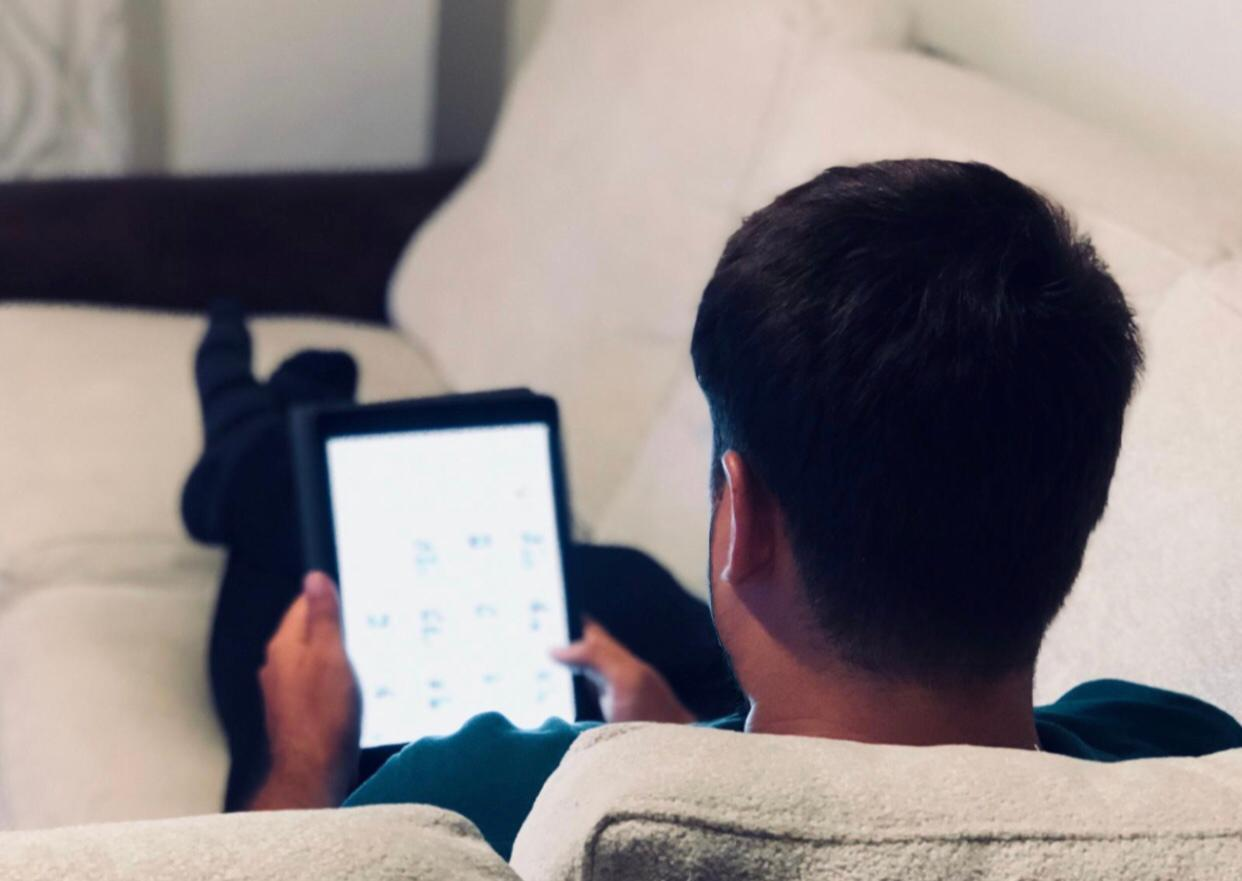
\includegraphics[width=0.8\textwidth]{fig-001.jpg}
 \caption{Student viewing the contents outside the school environment.}
 \label{fig1}
 \source{from the authors.}
\end{figure}

The other two remaining groups developed the different sessions through augmented reality, through the use of tablets to read different templates provided by the teacher in the classroom with QR codes. These templates allowed access to information about the content to be taught (\Cref{fig2}). In turn, they contained theoretical information so that students could consult, exercise demonstrations and extra information for advanced students.

\begin{figure}[htbp]
 \centering
 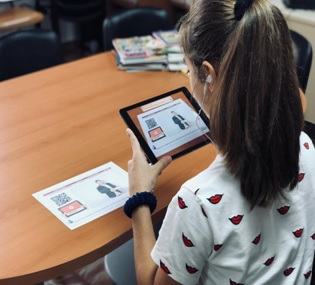
\includegraphics[width=0.8\textwidth]{fig-002.jpg}
 \caption{Student accessing information by reading the QR code.}
 \label{fig2}
 \source{from the authors.}
\end{figure}

In addition, a specific application was used on said contents, called Geometry. This application allows you to interact with the figures, view all their faces and solve questions and problems (\Cref{fig3}). In this way, the students were able to get in touch with their own content in 3 dimensions (3D) thanks to augmented reality technology. The application was used in class time as it allowed the explanation of content, the completion of tasks and their correction and automatic feedback.

\begin{figure}[htbp]
 \centering
 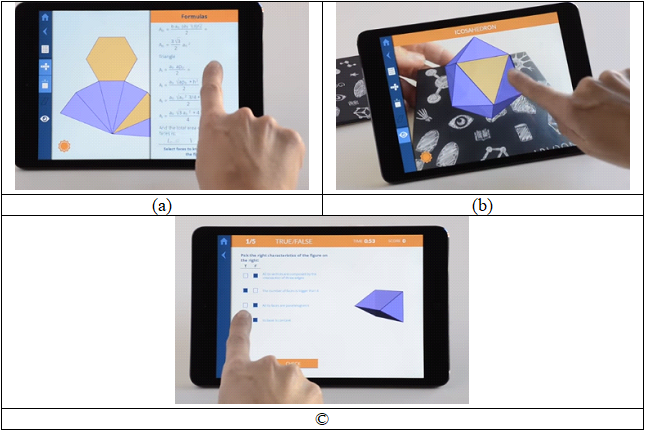
\includegraphics[width=0.8\textwidth]{fig3.png}
 \caption{Geometry application. Theoretical-practical information (a); Viewing and interaction in 3D of the figures (b); Assessment tasks (c).}
 \label{fig3}
 \source{from the authors.}
\end{figure}

In the different groups, the training intervention was developed by a single teacher, in order to avoid possible biases in the instructional action of different teachers. The assignment of the treatment (type of training action) to the group was carried out randomly. After carrying out the educational intervention, the data was collected using the questionnaire. Then they were analyzed with the statistical program and conclusions were drawn.

\section{Results}
In general, the data collected in table two shows the descriptive statistics developed in this study, show normal distribution parameters. The reason for choosing parametric tests is that the kurtosis and skewness are between -1.96 and +1.96, according to \textcite{joreskog2001}. Students in Secondary Education have shown a different response tendency, depending on the didactic method applied. Students who have developed an emerging methodology show averages ranging from 2.5 to 3, which shows a medium to high evaluation of this teaching procedure. The highest average is given by the teacher/learner ratio dimension, while the lowest average is given by the student/content ratio dimension. In contrast, students who have received training based on educative technology have also shown average values similar to those of the other group. In this case, there are four dimensions that exceed the average of 3. It can be determined that this method is generally valued by students as medium-high. The dimension with the highest average is motivation. On the other hand, among the various dimensions, class time is the one with the lowest value. Both groups developing the MS method and the group applying the ET method, no dispersion of response is shown. This is due to the fact that the standard deviation values are below 1. Also, it must be taken into account that kurtosis in both groups is mainly platykurtic, although occasionally, mesokurtic and leptokurtic kurtosis are observed (\Cref{tab2}).

\begin{table}[htpb]
\caption{Results achieved in the dimensions of research in EM and ET in Secondary Education.}
\label{tab2}
\centering
\small
\begin{tabular}{p{0.09\textwidth}p{0.12\textwidth}p{0.07\textwidth}p{0.08\textwidth}p{0.08\textwidth}p{0.09\textwidth}p{0.04\textwidth}p{0.04\textwidth}p{0.06\textwidth}p{0.06\textwidth}}
\toprule 
& & \multicolumn{4}{c}{Likert Scale emph{n (\%)}} & \multicolumn{4}{c}{Parameters}
\\ 
& Dimensions & None & Few & Enough & Completely & M & SD & Skw & Kme
\\
\midrule
\arrayrulecolor[gray]{.7}
\multirow{10}{=}{Emerging methodology (EM)}	& Motivation & 7(11.9) & 18(30.5) & 23(39) & 11(18.6) & 2.64 & .924 & -.169 & -.754
\\
%\cmidrule{2-10}
& Teacher-student	& 3(5.1) & 13(22) & 23(39) & 20(33.9) & 3.02 & .881 & -.504 & -.548
\\ 
%\cmidrule{2-10}
& Student-content & 8(13.6) & 20(33.9) & 19(32.2) & 12(20.3) & 2.59 & .967 & -.036 & -.941
\\
%\cmidrule{2-10}
& Student-student & 5(8.5) & 20(33.9) & 24(40.7) & 10(16.9) & 2.66 & .863 & -.104 & -.602
\\
%\cmidrule{2-10}
& Autonomy & 7(11.9) & 15(25.4) & 20(33.9) & 17(28.8) &	2.80 & .996 & -.332 & -.936
\\
%\cmidrule{2-10}
& Collaboration	& 8(13.6) & 18(30.5) & 21(35.6) & 12(20.3) & 2.63 & .963 & -.135 & -.897
\\
%\cmidrule{2-10}
& Deepening	& 2(3.4) & 14(23.7) & 28(47.5) & 15(25.4) & 2.95 & .797 & -.330 & -.389
\\
%\cmidrule{2-10}
& Resolution & 9(15.3) & 13(22) & 27(45.8) & 10(16.9) & 2.64 & .943 & -.369 & -.685
\\
%\cmidrule{2-10}
& Classtime	& 3(5.1) & 14(23.7) & 32(54.2) & 10(16.9) &	2.83 & .769 & -.403 & .067
\\
%\cmidrule{2-10}
& Ratingsa & 6(10.2) & 10(16.9) & 27(45.8) & 16(27.1) & 2.90 & .923 & -.610 & -.314
\\ 
\midrule
\multirow{10}{=}{Educative technology (ET)} & Motivation & 2(3.5) & 11(19.3) & 24(42.1) & 20(35.1) & 3.09 & .830 & -.557 & -.349
\\
%\cmidrule{2-10}
& Teacher-student & 9(15.8) & 16(28.1) & 23(40.4) & 9(15.8) & 2.56 & .945 & -.183 & -.815
\\
%\cmidrule{2-10}
& Student-content & 3(5.3) & 12(21.1) & 24(42.1) & 18(31.6) & 3.00 & .866 & -.513 & -.411
\\
%\cmidrule{2-10}
& Student-student & 2(3.5) & 9(15.8) & 31(54.4) & 15(26.3) & 3.04 & .755 & -.574 & .357
\\
%\cmidrule{2-10}
& Autonomy	& 8(14) & 21(36.8) & 20(35.1) & 8(14) & 2.49 & .909 & .027 & -.732
\\
%\cmidrule{2-10}
& Collaboration	& 9(15.8) & 12(21.1) & 23(40.4) & 13(22.8) & 2.70 & .999 & -.361 & -.866
\\
%\cmidrule{2-10}
& Deepening	& 10(17.5) & 16(28.1) & 22(38.6) & 9(15.8) & 2.53 & .966 & .139 & -.903
\\
%\cmidrule{2-10}
& Resolution & 3(5.3) & 12(21.1) & 22(38.6) & 20(35.1) & 3.04 & .886 & -.549 & -.501
\\
%\cmidrule{2-10}
& Classtime	& 9(15.8) & 20(35.1) & 20(35.1) & 8(14) & 2.47 & .928 & .010 & -.797
\\
%\cmidrule{2-10}
& Ratingsa & 8(14) & 18(31.6) & 22(38.6) & 9(15.8) & 2.56 & .926 & -.116 & -.771
\\
\arrayrulecolor{black}
\bottomrule
\end{tabular}
\centering
\source{from the authors.}
\notes{Established grade group (None: 1-4.9; Few: 5-5.9; Enough: 6-8.9; Completely: 9-10).}
\end{table}

The comparison of means shows differences in most study dimensions when taken individually. If the overall mean for each of the groups is taken into account, the ratings are similar, with the group that developed the MS method being much higher. The motivation, student-content, student-student and resolution dimensions were rated better by the ET group than by the MS group. Moreover, the autonomy, teacher-student, classtime, deepening and ratings dimensions were better evaluated by the EM group than by the ET group (\Cref{fig4}).

\begin{figure}[htbp]
 \centering
 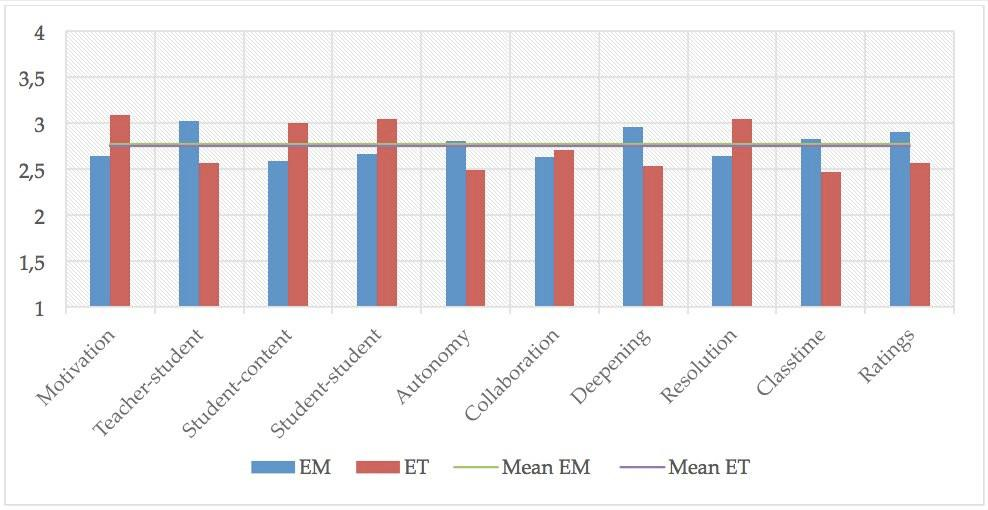
\includegraphics[width=0.75\textwidth]{fig-004.jpg}
 \caption{Comparative between experimental group and control group.}
 \label{fig4}
 \source{from the authors.}
\end{figure}

The results presented in \Cref{tab3} show the degree of independence in both pedagogical methods. These data are obtained after applying the Student's t-statistic method, specifically the independent samples method. Significant relationships are present in these data, in particular in motivation and teachers-student dimensions, although with different trends. The first one is in favour of the ET group and the second one in favour of the EM group. The dimensions resolution, student-content, deepening, student-student and rating show significant relationships. In this case, the student-student, student-content and resolution dimensions are in favour of the ET group. In contrast, deepening is in favour of the EM group. The biserial correlation indicates a medium-low associative strength in all study dimensions. Furthermore, for all dimensions of the study, the effect size is very low.

\begin{table}[htpb]
\caption{Study of the value of independence between experimental group and control group.}
\label{tab3}
\centering
\begin{tabular}{lS[table-format=1.3]SSS[table-format=3]SS}%{llllll}
\toprule
Dimensions & {$\mu$} & {$(X_1 - X_2)$} & {$t_{n1+n2-2}$} & {$df$} & {$d$} & {$r_{xy}$} \\
\midrule
Motivation & -.444 & {(2.64-3.09)} & -2.718** & 114 & -.009 & .247
\\
Teacher-student & .456 & {(3.02-2.56)} & 2.687** & 114 & -.014 & -.244
\\
Student-content & -.407 & {(2.59-3.00)} & -2.384* & 114 & -.014 & .218
\\
Student-student & -.374 & {(2.66-3.04)} & -2.481* & 114 & -.039 & .226
\\
Autonomy & .305 & {(2.80-2.49)} & 1.723 & 114 & .030 & -.159
\\
Collaboration & -.075 & {(2.63-2.70)} & -.410 & 114 & -.037 & .038
\\
Deepening & .423 & {(2.95-2.53)}	& 2.576* & 114 & -.030 & -.235
\\
Resolution & -.391 & {(2.64-3.04)} & -2.301*	& 114 & .027 & .211
\\
Classtime & .357 & {(2.83-2.47)} & 2.258* & 114 & .002 & -.207
\\
Ratingsa & .337 & {(2.90-2.56)} & 1.962	& 114 & .033 & -.181
\\
\bottomrule
\end{tabular}
\centering
\source{from the authors.}
\notes{* Significant correlation (0.05 level) \hspace{2em}
** Very significant correlation (0.01 level)\\
n.s. Correlation not significant\\
a. Established grade group (None: 1-4.9; Few: 5-5.99; Enough: 6-8.99; Completely: 9-10)}
\end{table}

\section{Discussion and Conclusions}
This study has comparatively analyzed the effectiveness of flipped learning and AR in Mathematics class. The need to analyze both elements within the training actions is based on the importance of optimizing and renewing current education. Updating education is essential for teachers to carry out methodologies adapted to current socio-educational needs \cite{area2016, larionova2018, pereira2019}. The flipped learning methodology \cite{sanchez2019, zainuddin2019} and the use of AR in educational contexts \cite{cabero2019, lorenzo2018} represent two fundamental resources to contribute to the optimization of current education. This issue also becomes fundamental within the mathematics classroom, where the use of flipped learning \cite{adams2018, amstelveen2019} and AR \cite{cahyono2020} has gained prominence in recent years.

The results obtained in this study coincide with those obtained in other similar investigations that analyze the same topic (Emerging methodology) in the mathematics classroom. In this way, it has been obtained that this emerging methodology generates an improvement in the participation, performance and grades of students in the mathematics area \cite{adams2018, amstelveen2019, sun2018}. Likewise, this study coincides with other investigations in the verification of an improvement in the autonomy of the student \cite{salas2019, touron2015} and a greater use of time in the classroom \cite{longcummins2017}.

Likewise, the results obtained regarding the use of AR (Educative technology) are similar to those found in the scientific literature. In this way, it has been obtained that the use of AR generates a significant increase in student motivation \cite{caberollorentegutierrez2017}, and facilitates access to the didactic contents \cite{barroso2017, marincabero2018}. On the other hand, there has also been an improvement in the interrelationships of the students within the classroom \cite{caberollorentemarin2017} and an increase in their ability to explore learning in their search for solutions to the problems raised \cite{fombonavazquez2017}. 

In conclusion, both the application of an emerging methodology based on flipped learning and the use of educational technology with AR contributes positively to the optimization of teaching and learning processes. The use of the flipped learning model as an emerging methodology has contributed positively to the interrelation of students with teachers, to the improvement of their degree of autonomy, to the deepening of learning, to the use of time in the classroom and to significant improvement in ratings. On the other hand, the use of AR as a techno-educational resource has led to significant improvements in student motivation, in access to didactic content, in the interrelationships between students and in their ability to solve problems.

For all the above, this research presents an interesting added value for the scientific community and for the teaching community, since they open the way for research in a field in need of this type of study. Analyzing in a comparative way the effects of active methodologies in general, and of flipped learning and AR in particular, allows increasing the information field of its results in learning process. The updating of current teaching must be nourished by these analyzes in order to implement the didactic methodologies that best adapt to the needs of the students.

A limitation of this research is related to the scope of the results obtained, which should be taken with caution. This is an exploratory study with a small sample size, so the results are not generalizable. Likewise, the results obtained do not reflect the specific contribution percentage of the turning over of the learning moments, the active role of the student, the use of techno-pedagogical resources or the use of AR. In addition, the discussion of the results obtained with the scientific literature is complex, due to the scarcity of studies that comparatively analyze the incidence of flipped learning and AR in the teaching and learning processes.

An interesting future line of research is to carry out an analysis of the effects of an optimization plan of the flipped learning model and of the application of AR in the Mathematics class, based on the development of a holistic analysis (strengths, weaknesses, opportunities and threats). Likewise, it is proposed to analyze in a combined way the effect of other active methodologies within the learning process in the Mathematics class. Finally, in relation to the new socio-educational context starring covid-19, it is proposed to investigate the possibility of applying AR and flipped learning methodology with limited availability of the face-to-face classroom.







\printbibliography\label{sec-bib}
% if the text is not in Portuguese, it might be necessary to use the code below instead to print the correct ABNT abbreviations [s.n.], [s.l.] 
%\begin{portuguese}
%\printbibliography[title={Bibliography}]
%\end{portuguese}

\end{document}
